\documentclass[screen, compress]{beamer}
\usepackage[T1]{fontenc}
\usepackage[utf8]{inputenc}
\usepackage{graphicx}
\usepackage{wrapfig}
\usetheme{Warsaw}

\title[TDT4215 project presentation]{TDT4215: Web-intelligence\\Group 1 project presentation}

\author[Terje Snarby, Even Wiik Thomassen and Weilin Wang]{Group 1\\
Terje Snarby\\
Even Wiik Thomassen\\
Weilin Wang%
}

%Norges teknisk-naturvitenskapelige universitet
\institute[NTNU]{
\includegraphics[width=0.75\textwidth,height=0.22\textheight]{img/ntnu}}

\date{\today}

\begin{document}

%=====================
\section{Introduction}
%=====================

%------------------
\subsection{Group 1}
\begin{frame}
%------------------
\titlepage
\end{frame}

%---------------------------------
\subsection{System architecture}
\begin{frame}{System architecture}
%---------------------------------
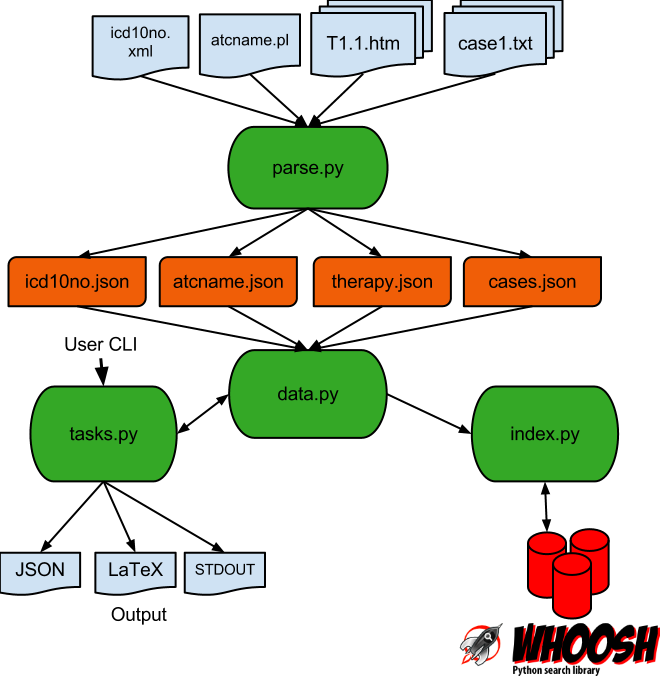
\includegraphics[width=\textwidth,height=0.92\textheight]{img/system_architecture2}
\end{frame}


%============================
\section{Methods and results}
%============================

%--------------------------
\subsection{Task 1 and 2}
\begin{frame}{Task 1 and 2}
%--------------------------
We've used Whoosh + BMF25F something something
\end{frame}


%--------------------
\subsection{Task 3}
\begin{frame}{Task 3}
%--------------------
\end{frame}


%--------------------
\subsection{Task 4}
\begin{frame}{Task 4}
%--------------------
\end{frame}


%--------------------
\subsection{Task 6}
\begin{frame}{Task 6}
%--------------------
\end{frame}


%====================
\section{Evaluations}
%====================

%--------------------------
\subsection{Oppsummering}
\begin{frame}{Oppsummering}
%--------------------------
\end{frame}


%------------------------
\subsection{Questions?}
\begin{frame}{Questions?}
%------------------------
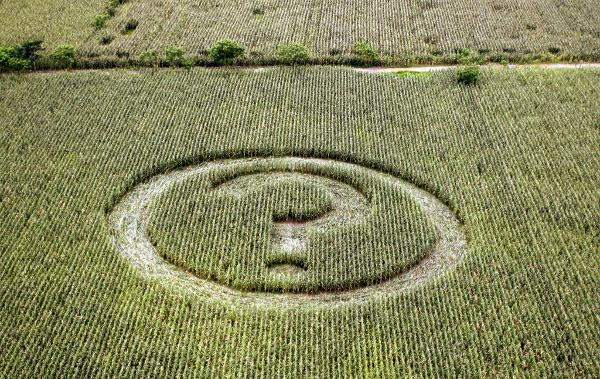
\includegraphics[width=\textwidth]{img/any-questions}
\end{frame}

\end{document}

